\section{Durchführung}
\label{sec:Durchführung}

\subsection{Untersuchung der Filterkurve des Selektivverstärkers}
Bei einer Güte von $Q = \num{100}$ wird die Filterkurve des Selektivverstärkers
untersucht. Bei einer konstanten Eingangsspannung $U_\text{E} = \SI{100}{\milli\volt}$
wird die Ausgangsspannung $U_\text{A}$ bei variierender Frequenz gemessen.
Die Frequenz wird auf $\nu = \SI{20}{\kilo\hertz}$ gestellt und in $\SI{1}{\kilo\hertz}$
Schritten auf $\SI{40}{\kilo\hertz}$ erhöht. In einem Bereich von plus und minus 
$\SI{1}{\kilo\hertz}$ vom Spannungsmaximum wird noch einmal genauer in $\SI{0.1}{\kilo\hertz}$
Schritten gemessen.

\noindent Eine theoretische Filterkurve eines Selektivverstärkers ist in Abb. 
\ref{abb:filterkurve} dargestellt.


\subsection{Suszeptibilität mittels Spannungsverhältnis bzw. Widerstandsverhältnis}
Es wird die Schaltung aus Abb. \ref{abb:schaltbild} nachgebaut.

\begin{figure}
    \centering
    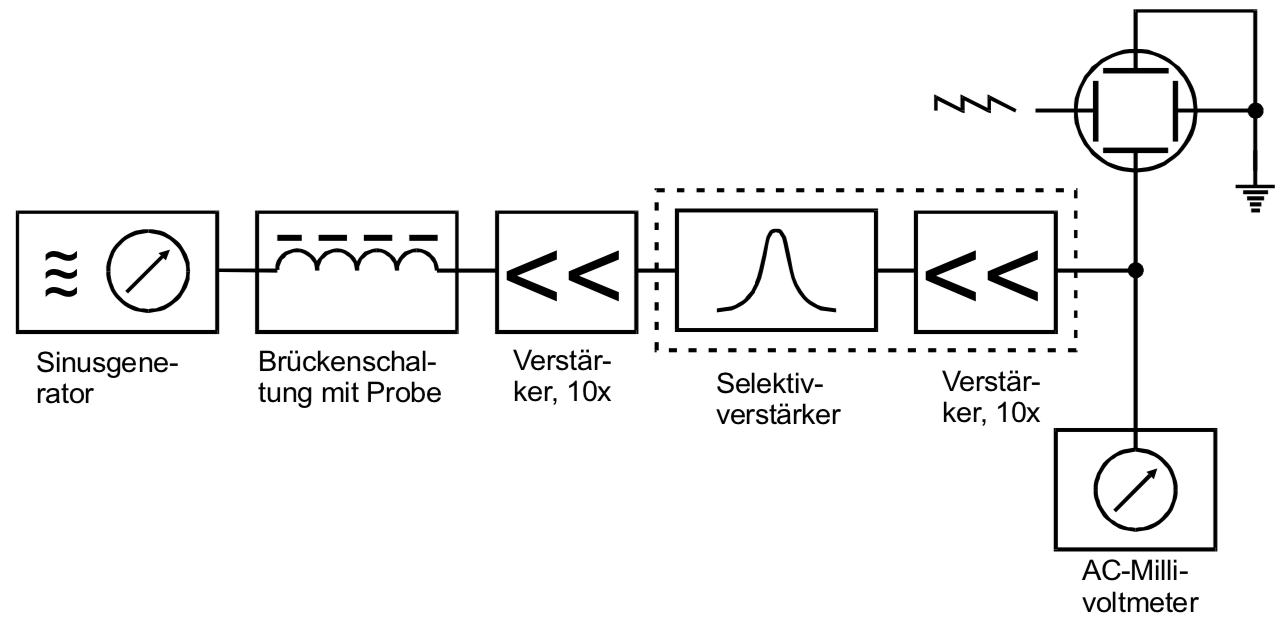
\includegraphics[width=12cm, height=6cm]{build/schaltbild.png}
    \caption{Schaltung zur Bestimmung der Suszeptibilität. \cite{V606}}
    \label{abb:schaltbild}
\end{figure}

\noindent Die Brückenspannung wird mittels der Widerstände auf ihr Minimum abgeglichen.
Die Probe wird in die Brückenschaltung geschoben. Die jetzt angezeigte Brückenspannung
wird aufgenommen. Anschließend wird die Brückenspannung mit dem Widerstand wieder auf
ihr Minimum abgeglichen. Der Wert des Widerstandes wird ebenfalls aufgenommen.
Das Ganze wird für alle vier Proben drei mal durchgeführt.

\noindent Aus der Änderung der Brückenspannung $\Delta U_\text{Br}$ bzw. aus der 
Änderung des Widerstandes $\Delta R$ kann die Suszeptibilität $\chi$ von Oxiden 
Seltener-Erd-Verbindungen bestimmt werden.